\documentclass[a4paper,12pt]{article}
\usepackage{amsmath,amssymb}
\usepackage{graphicx}
\usepackage{geometry}
\geometry{margin=1in}
\usepackage{enumitem}
\usepackage{booktabs}
\usepackage{parskip}
\setlength{\parindent}{0pt}
\usepackage{float}
\usepackage[absolute,overlay]{textpos}

\begin{document}

\title{\textbf{Battle of the Sexes: Game Analysis\\
    \small Game Theory Final Project}}

\author{Mostafa Hazem 2205174, Meray Mohsen 2205060, Mohamed Ghonem 2205050, \\ 
Basmala Ahmed 2205192, Malak Hashem 2205090, Zyad Yasser Fawzy 2205022}
\date{May 2025}
\maketitle

\begin{textblock*}{3cm}(15.7cm,0.8cm)
    
\includegraphics[width=2.625cm]{ANU_LOGO.jpg}
\end{textblock*}

\section{Story}
A man and a woman want to get together for an evening of entertainment, but they have no means of communication. They can either go to the ballet or the fight. The man prefers going to the fight, while the woman prefers going to the ballet. However, both prefer being together rather than being alone.


\section{Game Tree}
The extensive form of the game is depicted below, showing the sequential decision-making process. The dashed line from Woman's first to second decision node indicates simultaneous moves.

\begin{figure}[H]
\centering
\includegraphics[width=0.8\textwidth]{tree_plot.png}
\caption{Game Tree for Battle of the Sexes}
\end{figure}

\section{Normal Form Game}
The normal form representation is shown below, summarizing the payoffs in a matrix format.

\begin{figure}[H]
\centering
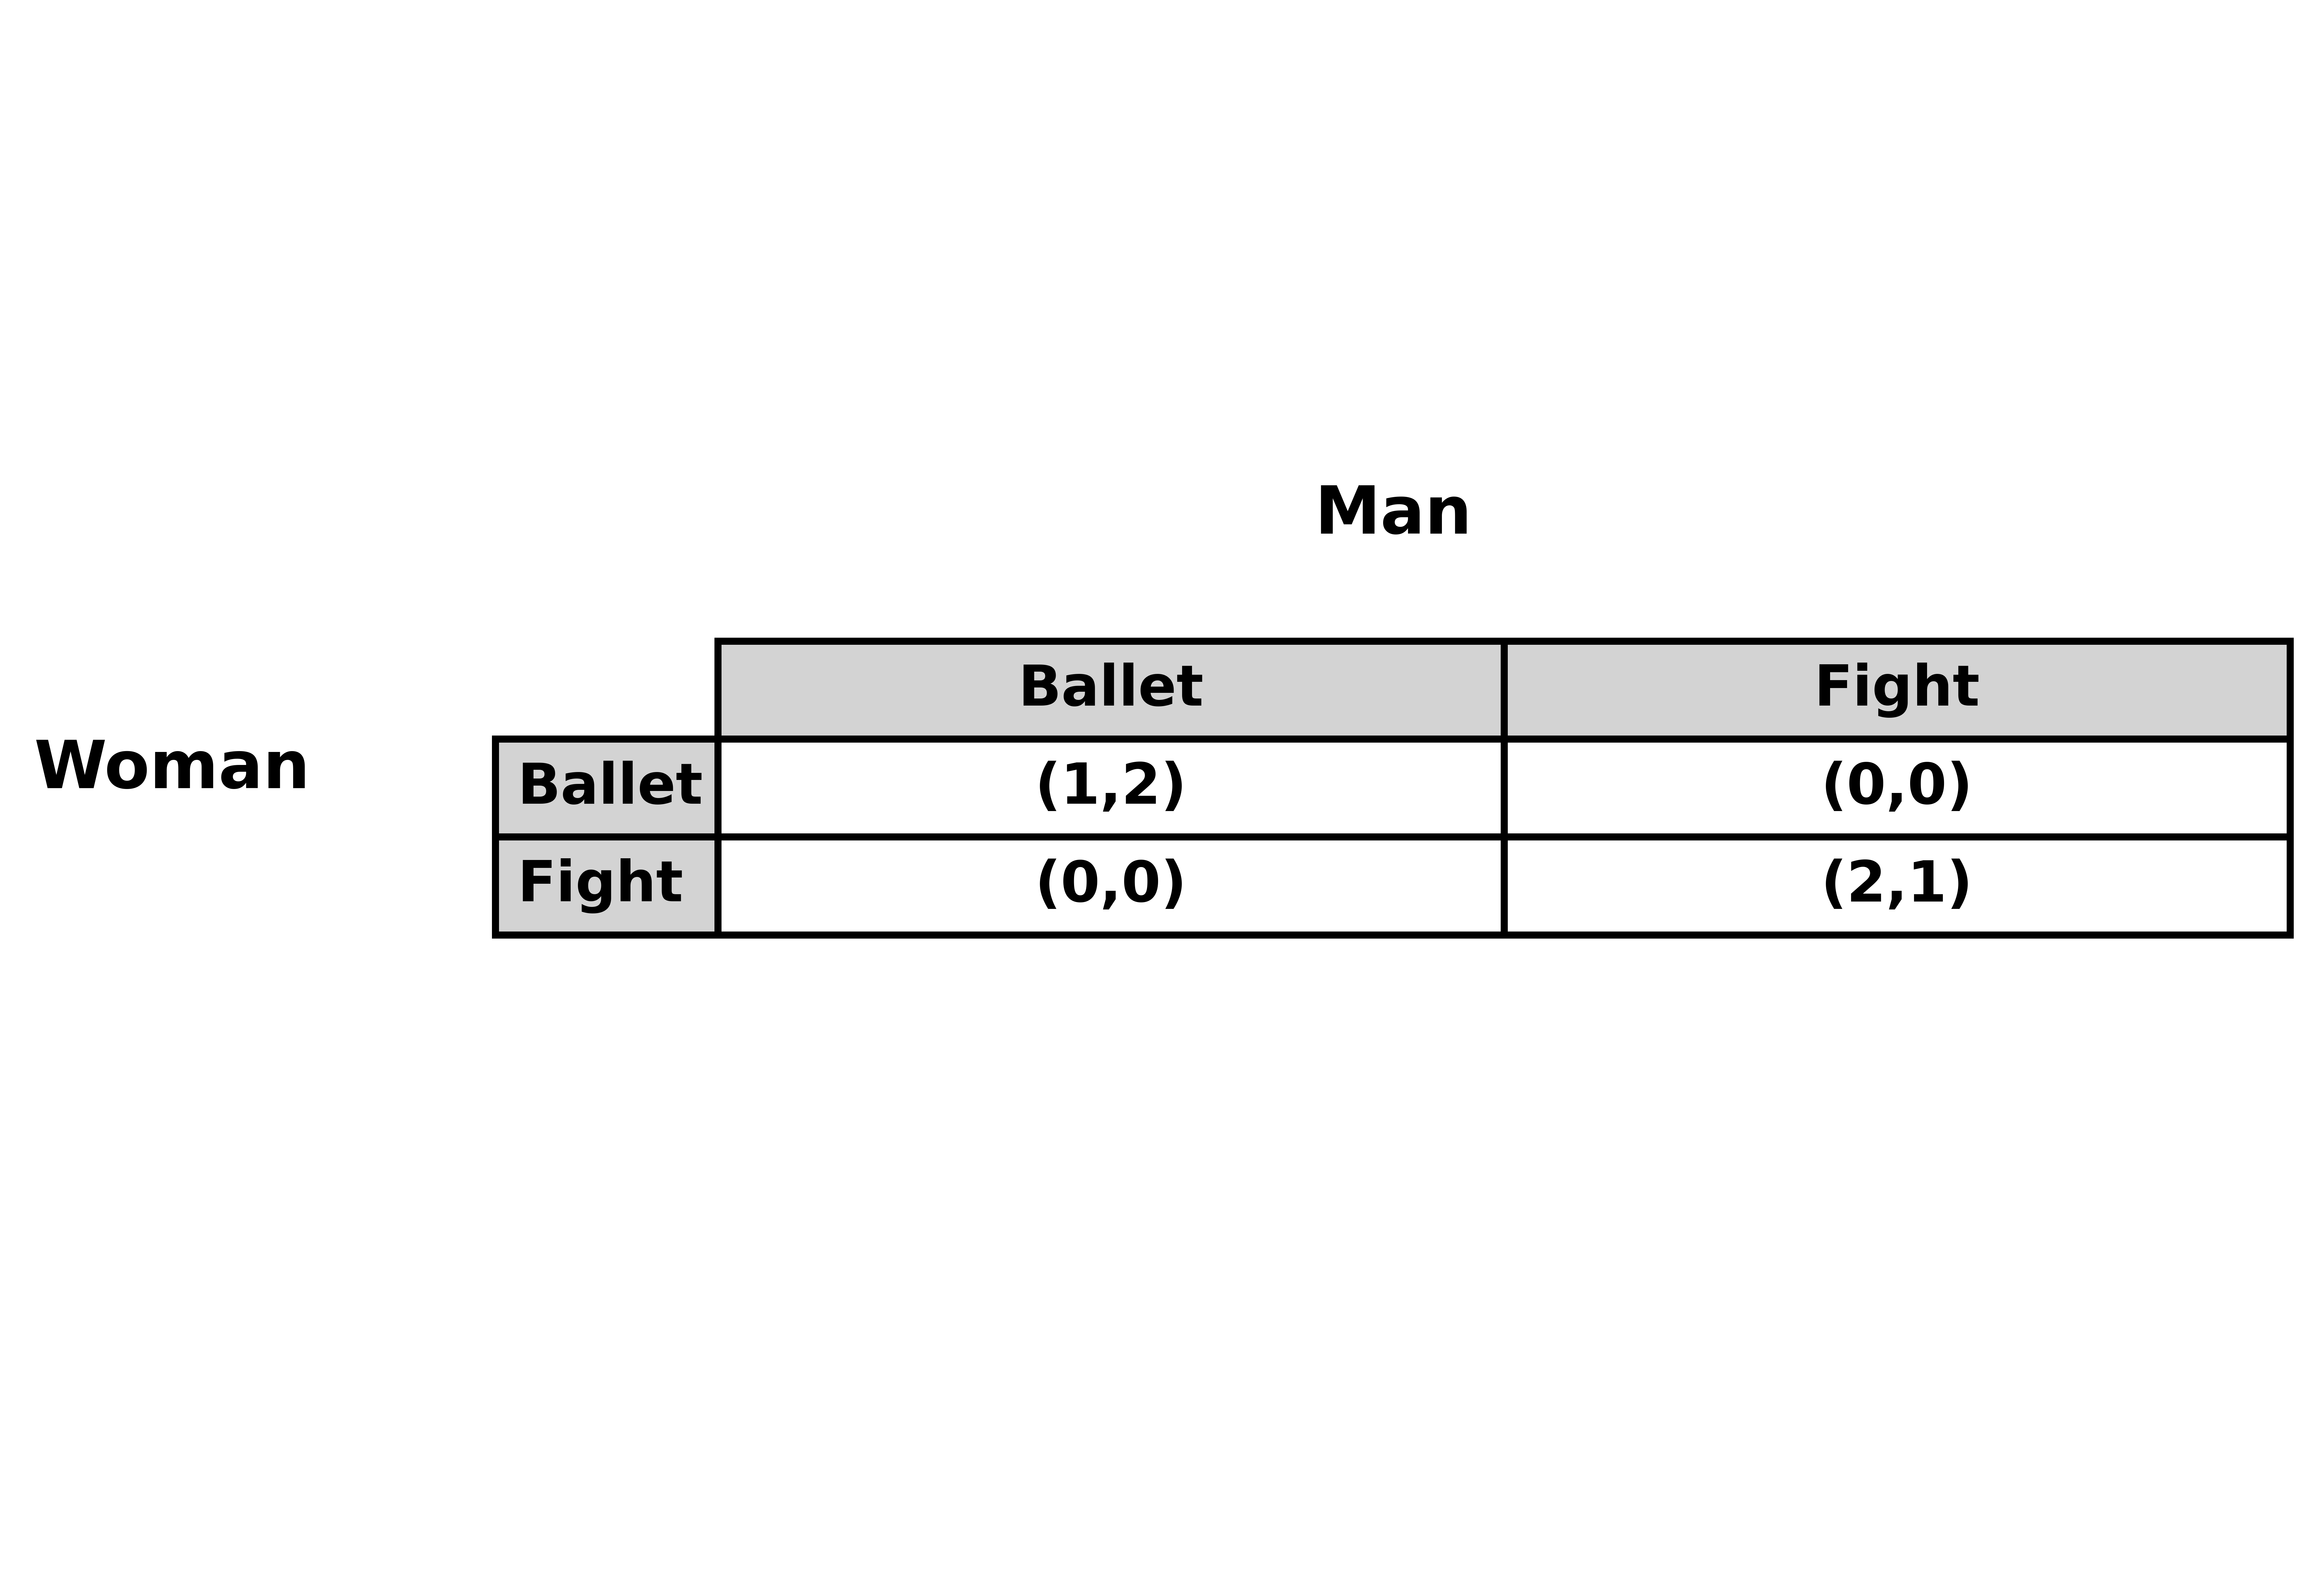
\includegraphics[width=0.5\textwidth]{payoff_table.png}
\caption{Normal Form Payoff Matrix}
\end{figure}
\section{Game Analysis}
The payoff matrix for the Battle of the Sexes game is shown below, with payoffs given as (Man, Woman):

\begin{center}
\begin{tabular}{c|cc}
\toprule
Man \textbackslash\ Woman & Ballet & Fight \\
\midrule
Ballet & (1,2) & (0,0) \\
Fight & (0,0) & (2,1) \\
\bottomrule
\end{tabular}
\end{center}

\subsection{Dominated Strategies}
To determine if any strategies are strictly dominated, we compare the payoffs for each player's strategies.

\begin{itemize}
\item \textbf{Man}: For Ballet, payoffs are 1 (if Woman plays Ballet) and 0 (if Fight). For Fight, payoffs are 0 (if Ballet) and 2 (if Fight). Since 1 $> 0$ in one case and Fight yields 2 $> 0$ in another, neither strategy is dominated.
\item \textbf{Woman}: For Ballet, payoffs are 2 (if Man plays Ballet) and 0 (if Fight). For Fight, payoffs are 0 (if Ballet) and 1 (if Fight). Since 2 $> 0$ and Fight yields 1 $> 0$, neither strategy is dominated.
\end{itemize}

\textbf{Result}: No strictly dominated strategies exist.

\subsection{Best Responses}
We identify each player's best response to the other's strategies.

\begin{itemize}
\item \textbf{Man}:
\begin{itemize}
\item If Woman plays Ballet: Payoffs are Ballet: 1, Fight: 0. Best response: Ballet ($1 > 0$).
\item If Woman plays Fight: Payoffs are Ballet: 0, Fight: 2. Best response: Fight ($2 > 0$).
\end{itemize}
\item \textbf{Woman}:
\begin{itemize}
\item If Man plays Ballet: Payoffs are Ballet: 2, Fight: 0. Best response: Ballet ($2 > 0$).
\item If Man plays Fight: Payoffs are Ballet: 0, Fight: 1. Best response: Fight ($1 > 0$).
\end{itemize}
\end{itemize}

\subsection{Rationalizable Strategies}
Rationalizable strategies are those that survive iterated elimination of strictly dominated strategies or are best responses to some beliefs about the opponent's strategies.

\begin{itemize}
\item \textbf{Check for strictly dominated strategies}:
\begin{itemize}
\item For Man: Ballet yields payoffs 1 (if Woman plays Ballet) and 0 (if Fight), while Fight yields 0 (if Ballet) and 2 (if Fight). Since 1 $> 0$ but 0 $< 2$, neither strategy is strictly dominated.
\item For Woman: Ballet yields payoffs 2 (if Man plays Ballet) and 0 (if Fight), while Fight yields 0 (if Ballet) and 1 (if Fight). Since 2 $> 0$ but 0 $< 1$, neither strategy is strictly dominated.
\end{itemize}
No strategies are eliminated in the first iteration, and since the strategy sets remain unchanged, no further eliminations occur.
\item \textbf{Best response analysis}:
\begin{itemize}
\item For Man: If Man believes Woman plays Ballet with probability $q$, his expected payoffs are:
\begin{align*}
\text{Ballet}: q \cdot 1 + (1-q) \cdot 0 = q \\
\text{Fight}: q \cdot 0 + (1-q) \cdot 2 = 2(1-q)
\end{align*}
Ballet is a best response if $q \geq 2(1-q)$, i.e., $q \geq \frac{2}{3}$. Fight is a best response if $2(1-q) \geq q$, i.e., $q \leq \frac{2}{3}$. Both strategies are best responses for some $q \in [0,1]$.
\item For Woman: If Woman believes Man plays Ballet with probability $p$, her expected payoffs are:
\begin{align*}
\text{Ballet}: p \cdot 2 + (1-p) \cdot 0 = 2p \\
\text{Fight}: p \cdot 0 + (1-p) \cdot 1 = 1-p
\end{align*}
Ballet is a best response if $2p \geq 1-p$, i.e., $p \geq \frac{1}{3}$. Fight is a best response if $1-p \geq 2p$, i.e., $p \leq \frac{1}{3}$. Both strategies are best responses for some $p \in [0,1]$.
\end{itemize}
\end{itemize}

\textbf{Result}: Since no strategies are eliminated and all strategies are best responses to some beliefs, the rationalizable strategies are \{Ballet, Fight\} for Man and \{Ballet, Fight\} for Woman.

\subsection{Expected Payoffs}
Let Man play Ballet with probability $p$ and Fight with $1-p$, and Woman play Ballet with probability $q$ and Fight with $1-q$.

\begin{itemize}
\item \textbf{Man's expected payoff}:
\[
E_M = q \cdot 1 + (1-q) \cdot 0 + (1-p) \cdot [q \cdot 0 + (1-q) \cdot 2] = q + 2(1-p)(1-q)
\]
\item \textbf{Woman's expected payoff}:
\[
E_W = p \cdot 2 + (1-p) \cdot 0 + (1-q) \cdot [p \cdot 0 + (1-p) \cdot 1] = 2p + (1-p)(1-q)
\]
\end{itemize}

\subsection{Pure Strategy Nash Equilibria}
A pure strategy Nash equilibrium occurs where no player can improve their payoff by unilaterally deviating.

\begin{itemize}
\item \textbf{(Ballet, Ballet)}: Man gets 1 (vs. 0 if Fight), Woman gets 2 (vs. 0 if Fight). Stable.
\item \textbf{(Ballet, Fight)}: Man gets 0 (prefers Fight for 2), Woman gets 0 (prefers Ballet for 1). Unstable.
\item \textbf{(Fight, Ballet)}: Man gets 0 (prefers Ballet for 1), Woman gets 0 (prefers Fight for 2). Unstable.
\item \textbf{(Fight, Fight)}: Man gets 2 (vs. 0 if Ballet), Woman gets 1 (vs. 0 if Ballet). Stable.
\end{itemize}

\textbf{Result}: Pure Nash equilibria are (Ballet, Ballet) and (Fight, Fight).

\subsection{Mixed Strategy Nash Equilibrium}
In a mixed strategy Nash equilibrium, each player chooses probabilities to make the other indifferent.

\begin{itemize}
\item \textbf{Man's indifference}: Woman chooses $q$ such that Man's expected payoffs from Ballet and Fight are equal.
\begin{align*}
&\text{Ballet}: q \cdot 1 + (1-q) \cdot 0 = q \\
&\text{Fight}: q \cdot 0 + (1-q) \cdot 2 = 2(1-q) \\
&q = 2(1-q) \\
&q = 2 - 2q \\
&3q = 2 \\
&q = \frac{2}{3}
\end{align*}
\item \textbf{Woman's indifference}: Man chooses $p$ such that Woman's expected payoffs from Ballet and Fight are equal.
\begin{align*}
&\text{Ballet}: p \cdot 2 + (1-p) \cdot 0 = 2p \\
&\text{Fight}: p \cdot 0 + (1-p) \cdot 1 = 1-p \\
&2p = 1-p \\
&3p = 1 \\
&p = \frac{1}{3}
\end{align*}
\end{itemize}

At the mixed NE, Man plays Ballet with $p = \frac{1}{3}$, Fight with $1-p = \frac{2}{3}$; Woman plays Ballet with $q = \frac{2}{3}$, Fight with $1-q = \frac{1}{3}$. Expected payoffs are:
\begin{itemize}
\item Man: $E_M = q = \frac{2}{3}$
\item Woman: $E_W = 2p = 2 \cdot \frac{1}{3} = \frac{2}{3}$
\end{itemize}

\end{document}
